\documentclass[11pt]{article}
\usepackage{imakeidx}
\usepackage{geometry}
\usepackage{amsmath}
\usepackage{graphicx}
\graphicspath{{images/}}

\usepackage{amsfonts}
\usepackage{mathtools}
\geometry{a4paper,
total={170mm, 257mm},
left = 30mm,
right = 30mm,
bottom = 30mm,
top = 30mm
}
\title{Models of Computation \linebreak Revision Notes}
\author{James Brown}
\makeindex

\newtheorem{theorem}{Theorem}
\newtheorem{corollary}{Corollary}
\newtheorem{definition}{Definition}

\newcommand\leqp{\stackrel{\mathclap{\normalfont\mbox{P}}}{\leq}}

\begin{document}
	\pagenumbering{gobble}
	\maketitle
	\newpage
	\tableofcontents
	\newpage
	\pagenumbering{arabic}
	
	\section{Introduction}
	These are notes I have written in preparation for the upcoming 2017 Models of Computation exam. This year the module was run by Paul Levy (P.B.Levy@cs.bham.ac.uk).
	\linebreak	
	This module is about problems and \textit{computers}. We ask ourselves:
	\begin{itemize}
		\item What problems can be solved on a computer?
		\item What problems can be solved on a computer with finitely many states?
		\item What problems can be solved on a computer with only finitely many states, but also a stack of unlimited size?
		\item What problems can be solved on a computer with only finitely many states, but also a tape of unlimited size that it can read and write to?
		\item What problems can be solved \textit{fast} on a computer?
		\item What does "fast" mean anyway?
		\item What does \textit{computer} mean anyway?
	\end{itemize}
	
	\section{Language Membership Problems and Regular Expressions}
	\subsection{Language Membership Problems}
	Suppose we have a set of characters $\Sigma$, which we will call the \textit{alphabet}\index{alphabet}. A \textit{word}\index{word} is a finite sequence of characters, and we write $\Sigma^{*}$ for the set of all words. We can \textit{concatenate}\index{concatenate} words. A \textit{language}\index{language} is a set of words and a subset of $\Sigma^{*}$. Given a word, we want to know is it in the language or not? If we take an example alphabet ${a, b, c}$, here are some languages:
	\begin{itemize}
		\item All words which contain exactly 3 \textit{b}'s
		\item All words whose length is prime
		\item All words that have more \textit{b}'s than \textit{a}'s
		\item The words \textit{abc}, \textit{bac} and \textit{cb}
		\item No words at all
		\item The empty word
	\end{itemize}
	
	These examples are largely pretty useless, but this problem does have real world applications such as 
	\begin{itemize}
		\item Java has rules about what you can call a variable. Is the word read by the compiler a valid variable name?
		\item A user makes an account and enters a password, is it valid?
		\item A student has submitted code for an assignment, is it correct?
		\item Will this code crash when it's run?
	\end{itemize}
	
	In each one of these examples, we are provided with a word and we want to know whether it is an acceptable word. We want to make a computer tell us the answer.
	
	\subsection{Regex}
	\textbf{Regular Expressions}\index{regular expressions} are a useful notation for describing languages. We write Empty for the language consisting of no words (the empty set). We write \textit{a} for the language consisting of just the single-character a, and $\epsilon$ for the language consisting of just the empty word. If we have a language \textit{\textbf{L}} and \textit{\textbf{L'}}, we write \textit{\textbf{LL'}} for the set of words that are a concatenation of a word in \textit{\textbf{L}} and a word in \textit{\textbf{L'}}. We can also write \textit{\textbf{L|L'}} for the set of words that are in \textit{\textbf{L}} or \textit{\textbf{L'}} - the union of the two languages. We write \textit{\textbf{L*}} for the set of words that are a concatenation of some number of words in \textit{\textbf{L}} (some number may be 0).
	Just like arithmetic, regular expressions have precedence rules. $*$ has the highest precedence, then juxtaposition and then $|$.
	
	\par 
	Regular expressions in theoretical computer science mean an expression built from the above operations and nothing more. Regular expressions are used much more widely in programming with far more operations, but they cannot be used in the module. For example, $+$ is a very common operation but not available to us.
	
	
	\section{Finite State Automata}
	\subsection{Removing $\epsilon$ moves}
	Let $(Q, \delta, \text{Acc}, q_{0})$ be a NDFA with $\epsilon$-transitions. There is a slow a-transition from state $q$ to state $r$ when starting from state $q$ we can follow some number of $\epsilon$-transistions, then an a-transition and end in state $r$. A state $q$ is slowly accepting when starting from a state $q$ we can follow some number of $\epsilon$-transitions and reach and accepting state.
	
	\par To create a NDFA without $\epsilon$-transitions, we take the same states and the same initial state and make all slow transitions into normal transitions, and all slowly accepting states become accepting.
	
	\subsection{Determinisation}
	Given a NDFA $(Q, \delta, Acc, q_{0})$ we can form a DFA. The states in the DFA will be subsets of $Q$. From a state $U \subseteq Q$, when we input a, we take the set of states that we can reach by an a-transition from a state in $U$. Our accepting states are states which contain a state which is contained in Acc. The initial state stays the same as before.
	\subsection{Coverting a regular expression to a deterministic finite state automaton}
	Simply create a NDFA from the regular expression, remove $\epsilon$-moves and then determinise the automaton.
	\subsection{Converting a finite state automaton to a regular expression}
	Say we have states $\{0, 1, ..., n - 1\}$. For any state $i$ and $j$, and any $k \leq n$, we want a regex $E^{<k}_{i \rightarrow j}$ that accepts those words that take us from $i$ to $j$ with intermediate states all $<k$. We'll give two formulas: one for $E^{<0}_{i \rightarrow j}$ and one for $E^{k+1}_{i \rightarrow j}$.
	
	\begin{itemize}
		\item If $i \neq j$ and there are $a, b, c$-transitions from $i$ to $j$, then we define $E^{<0}_{i \rightarrow j}$ to be $a|b|c$. If there are no transitions, it's Empty.
		\item If there are $a, b, c$-transitions from $i$ to $i$, we define $E^{<0}_{i \rightarrow j}$ to be $\epsilon|a|b|c$. If there are no transitions, it's $\epsilon$.
		
		\item If $i \neq k$ and $j \neq k$ then define $E^{<k+1}_{i \rightarrow j}$ to be $E^{<k}_{i \rightarrow j}$ | $E^{<k}_{i \rightarrow k} {E^{<k}_{k \rightarrow k}}^{*} E^{<k}_{k \rightarrow j}$
		
		\item If $i \neq k$ then define $E^{<k+1}_{i \rightarrow k}$ to be $E^{<k}_{i \rightarrow k} {E^{<k}_{k \rightarrow k}}^{*}$
		
		\item If $j \neq k$ then define $E^{<k+1}_{k \rightarrow j}$ to be ${E^{<k}_{k \rightarrow k}}^{*} E^{<k}_{k \rightarrow j}$
		
		\item Define $E^{<k+1}_{k \rightarrow k}$ to be ${E^{<k}_{k \rightarrow k}}^{*}$
	\end{itemize}
	
	\section{Regular Languages}
	\begin{theorem}[Kleene's Theorem]
	A language is regular if and only if it is accepted by a finite state automaton.
	\end{theorem}
	 
	\subsection{Operations on regular languages}
	We use Kleene's theorem to prove that some languages are regular. Firstly, the complement of a regular language $L$ is also regular. To do this, we take the DFA $(Q, \delta, \text{Acc}, q_{0})$ which accepts $L$. We then take the automaton $(Q, \delta, Q\ \text{Acc}, q_{0})$. This automation recognises the complement of $L$, so the complement of $L$ must also be a regular language.
	
	\par 
	Secondly, the intersection of regular languages $L$ and $L'$ is regular, as it is the complement of the union of the complements of $L$ and $L'$.
	
	\subsection{Proving a language is not regular}
	\begin{theorem}[Myhill-Nerode Theorem]
	A language $L$ is not regular if and only if it has an infinite distinctive sequence.
	\end{theorem}
	
	Let $w$ and $w'$ be words, and $L$ a language. An $L$-distinguishing suffix for $w$ and $w'$ is a word $x$ such that either $wx \in L$ and $w'x \notin L$, or $wx \notin L$ and $w'x \in L$. For example, take the words \texttt{Wed} and \texttt{Tues}. An English-distinguishing suffix for these two words is \texttt{day} because \texttt{Wedday} is not and English word but \texttt{Tuesday} is.
	
	\par Suppose we have a DFA which recognises the language $L$. If words $w$ and $w'$ have an $L$-distinguishing suffix, then $w$ and $w'$ must take us to different states from the inital state. Now suppose we have four words, $w_{0}, w_{1}, w_{2}, w_{3}$ that are \textbf{distinctive}\index{distinctive} (meaning they all have distinguishing suffixes in relation to each other. The DFA to represent this language must have at least four states. Now suppose there is an infinite sequence of words $w_{0}, w_{1}...$ that is \textbf{distinctive}. There cannot be a DFA to represent this language, so by Kleene's theorem the language is not regular.
	
	\par 
	\textbf{Example}: Take the language $\{a^{n}b^{n} \;|\; n \in \mathbb{N}\}$. If we take all $a^{n}$ for each $n \in \mathbb{N}$, then for $m < n$, $b^{m}$ is a distinguishing suffix for $a^{m}$ and $a^{n}$. This is a distinctive infinite sequence, and the language is not regular.
	
	\subsubsection{The Pumping Lemma}
	
	\subsection{Context Free Languages}
	
	\section{Bisimulation and Minimisation}
	\subsection{Bisimilarity}
	Two states are \textbf{bisimilar}\index{bisimilarity} if and only if they accept the same language. Suppose $(Q, \delta, Acc)$ and $(Q', \delta ', Acc')$ are unpointed automata for the same alphabet $L$. A state $q_{0} \in Q$ is bisimilar to a state $q'_{0} \in Q'$ if and only if they accept the same language. In order to prove this, let $\mathcal{R}$ be a bisimulation. We will prove that for any word $w$, if $q \mathcal{R} q'$ then $q$ accepts $w$ if and only if $q'$ accepts $w$. This is by induction on $w$:
	
	\par 
	For the base case $w = \epsilon$:
	\begin{align*}
		&\;q \text{ accepts } \epsilon \\
			\leftrightarrow & \;q \text{ is accepting } \\ 
			\leftrightarrow & \;q' \text{ is accepting} \\
			\leftrightarrow & \;q' \text{ accepts } \epsilon
	\end{align*}
	
	For the inductive step where $w$ has a head (first character) $a$ and a tail $t$:
	\begin{align*}
		 &\;q \text{ accepts } a::t \\
			\leftrightarrow &\;\delta (q,a) \text{ accepts }  t \\ 
			\leftrightarrow &\;\delta'(q', a) \text{ accepts } t & \text{(by the inductive hypothesis)}\\
			\leftrightarrow &\;q' \text{ accepts } a :: t
	\end{align*}
	
	The easiest way to  construct a check for bisimilarity is to build a bisimulation (essentially a tree). From your pair of states, follow all outputs to new pairs of states. If any of the new pairs disagree on acceptance (one accepts and the other doesn't), then the original pair is not bisimilar as they both accept different languages. We stop building the tree down a branch if we see a pair of states that we have visited before, and conclude that the pair of states is bisimilar if we can't make any more moves that we haven't already seen before.
	\subsection{Minimisation}
	In order to minimise an automaton, there are two steps:
	\begin{enumerate}
		\item Throw away unreachable states
		\item Identify bisimilar states and merge the ones that are bisimilar
	\end{enumerate}
	
	The found minimal automaton will be unique (up to isomorphism).
		
		
	\section{The Halting Problem}
	In Computer Science there are many problems that we encounter. These all have an input (some string, a number, three strings etc.) and an output. Often this output is yes or no, but it may be a number or string or some other value. If a problem returns a yes or no result, then it is a decision problem\index{decision problem}. We have to draw a distinction between problems\index{problem} and instances\index{instance}. 'Is the word $abbab$ accepted by the regexp $ab*(ab*|b)$?' is an instance of a more general problem 'Is a word $w$ accepted by the regexp $ab*(ab*|b)$?'. Even more generally we could describe this problem as 'Given a word $w$ and a regexp $E$, is $w$ accepted by $E$?'.
	
	\par 
	Typically we want to consider problems which have a countably infinite set of acceptable inputs and acceptable outputs. Refer to Mathematical Techniques for Computer Science to see how we can ensure something is countably infinite. A problem can also be called a function\index{function}, and we can also describe it as a subset of the set of inputs. 
	\begin{itemize}
		\item Problem: given a positive integer, is it prime?
		\item The function that maps a positive integer to 'true' if it's prime and 'false' otherwise
		\item The subset of the set of positive integers consisting of all prime integers
	\end{itemize}
	If the set of inputs is the set of words over some alphabet, then the subset will be a language.
	
	\par
	\textbf{Key concepts:}
	\begin{itemize}
		\item A decision problem (a problem which returns a yes or no answer) is decidable if it can be solved on a computer.
		\item A function is computable if it can be computed on a computer.
		\item A subset of the set of inputs (a language) is decidable if the corresponding decision problem can be solved on a computer.
	\end{itemize}
	
	We still haven't come up with a definition for \textit{computer} yet! We get around this for now by saying a problem is 'Java-decidable' or 'Java-computable' for example, meaning that we can accomplish the task with a Java program.

	\subsection{Reducing a problem to another problem to solve the Halting problem}
	Suppose we have two problems - $P$ and $Q$. If we can show how to solve $Q$ using a black box which solves $P$ then we can say that we have reduced\index{reduce} the problem $Q$ to the problem $P$. If we can reduce $Q$ to $P$ then if $P$ is decidable\index{decidable}, $Q$ is decidable and if $Q$ is undecidable\index{undecideable}, $P$ is undecidable.
	
	\par
	Given a nullary Java method such as the one below, can we tell if it will terminate or not? We keep things simple by assuming integers are unbounded, no exceptions are thrown and any such method when called either terminates or hangs forever.
	\begin{verbatim}
		void f (){
		    ...
		}
	\end{verbatim}
	
	This is an example of the \textbf{Halting Problem}\index{halting problem}. Turing proved that the halting problem was undecidable. To prove this, we assume that it is decidable.
	
	\begin{enumerate}
		\item Consider the \textbf{unary halting problem}. Given a unary Java method
		\begin{verbatim}
			void f (String x) {
			    ...
			}
		\end{verbatim}			
		and a string $y$, does \texttt{f} terminate when called with $y$? We reduce the unary halting problem to the nullary one. Given the unary method \texttt{f} and a string $x$, obtain a nullary method \texttt{g} by taking the code of \texttt{f} and replacing \texttt{x} with $y$ - that is substitute in the argument values. Then, \texttt{g} terminates when called if \texttt{f} terminates when called with argument $y$. Since we assume the nullary halting problem is solvable, the unary one is too. This gives us a program
		\begin{verbatim}
			boolean haltcheck (String somemethod, String y)
		\end{verbatim}
		
		where \texttt{somemethod} is the body of a unary method. When we apply with $M$ and $y$ this method returns true when $M$ applied to $y$ terminates, otherwise it returns false.
	
	\item We build on this method further
		\begin{verbatim}
			void hangcheck (String somemethod, String y) {
			   if haltcheck(somemethod, y) {
			      while true {}
			   } else {
			      return;
			   }
			}
		\end{verbatim}	
		
		This method when applied to $M$ and $y$, hangs if $M$ applied to $y$ terminates, otherwise it returns.
				
	\item We build on this even further with a new program
		\begin{verbatim}
			void doublehang (String y) {
			    haltcheck(y, y)
			}
		\end{verbatim}
		
		This method when applied to $y$ (the body of the unary method), will hang if $y$ applied to $y$ terminates, otherwise it returns.
	
	\item Finally, let $z$ be the body of \texttt{doublehang}. We see that \texttt{doublehang}, when applied to $z$, terminates if and only if it hangs. This is a contradiction, so there cannot be any program which solves the halting problem.
	\end{enumerate}
	
	I find this method of solving the Halting problem very confusing, but here is an elegant solution: 
	\begin{verbatim}
	function halts(func) {
  // Insert code here that returns "true" if "func" halts and "false" otherwise.
}

function deceiver() {
  if(halts(deceiver))
    while(true) { }
}
	\end{verbatim}
		
	Assume deceiver halts, so it therefore enters an infinite loop and doesn't halt. Contradiction. Asssume deceiver doesn't halt. Deceiver never enters the loop and therefore does halt. Contradiction. The method halts can therefore never exist.
	
	\par 
	\textbf{Example:} Given a string s, is s the code of a Java program that either halts or contains \texttt{ccc}? 
	\par 
	Given the string $s$, we remove all occurances of \texttt{ccc} by replacing it with some other string to form \texttt{noccc\{s\}}. Now we know the $s$ is the code of a Java program that will halt if and only if \texttt{noccc\{s\}} is the code of a Java program that either halts or contains \texttt{ccc}. We have therefore reduced the Halting problem to our problem - if we could solve our problem we could solve the halting problem.
	\section{Properties of Code}
	Some property of a piece of code may be \textbf{trivial}\index{trivial} - it either holds for everything or it holds for nothing. Take the following code:
	
	\begin{verbatim}
	int f (int x) {
	    ...
	}
	\end{verbatim}
	
	We are interested if when applied to an integer $n$, it either hangs or returns an integer $y$ that is a factor of $3y$. This is a trivial property. Every trivial property is decidable.
	
	A property of a piece of code may be \textbf{semantic}\index{semantic}. Semantic properties concern the behaviour of a certain piece of code, but not how the behaviour is achieved. In this sense, if we view the piece of code as a black box then the semantic property depends purely on the inputs and outputs.
	
	\subsection{Rice's Theorem}
	\begin{theorem}[Rice's Theorem]
		Every non-trivial, semantic property of code is undecidable. We define a trivial property\index{trivial property} is one which either holds for everything or holds for nothing.
	\end{theorem}

	\par 
	To prove Rice's theorem, we let $\alpha$ be a non-trivial semantic property of code and let \texttt{alwayshang} be a piece of code that always hangs regardless of argument. We say that \texttt{alwayshang} doesn't satisfy $\alpha$, and since $\alpha$ is non-trivial we can say that there is another piece of code $C$ that does. For any nullary program $P$, we form $F(P)$ by inserting $P$ at the start of the code $C$.
	\begin{itemize}
		\item If $P$ terminates, then $F(P)$ has the same semantics as $C$. Because $\alpha$ is semantic and $C$ satisfies $\alpha$, $F(P)$ does too.
		\item If $P$ hangs, then $F(P)$ has the same semantics as \texttt{alwayshang}. Since $\alpha$ is semantic and \texttt{alwayshang} doesn't satisfy $\alpha$, $F(P)$ also doesn't.
	\end{itemize}
	
	In short, $P$ will terminate if and only if $F(P)$ satisfies $\alpha$. This means that if we can test for $\alpha$, we can also test whether $P$ terminates by testing if $F(P)$ satisfies $\alpha$. We've already proven that we can't prove $P$ terminates, so we must not be able to test for $\alpha$ - meaning $\alpha$ is undecidable\index{undecidable}.
	
	\par 
	We can use Rice's theorem to easily prove problems undecidable. If we want to check a piece of code for a property, we check if the property is trival (easy to do) and whether the property is semantic. If the property is non-trivial and semantic, the property is undecidable. 
	
	\par \textbf{Example:} Write a piece of code which takes a Java method. Return 'yes' if this code may be run with an argument which will cause an exception to be thrown. This is a semantic property as it directly refers to the behaviour of the method in the property. It is non-trivial as it does not hold for all possible methods, some have this property and others do not.
	
	\section{Turing Machines}
	In 1936, Alan Turing\index{alan turing} invented the \textbf{turing machine}\index{turing machine}. Turing machines are very simple computers, and have a very limited set of instructions that they can execute. They have finitely many states, but also have an infinite tape which they can compute upon. Because of this, a Turing machine is an idealized computer and can never exist in the physical world. Turing machines are very convenient for analysing the running times of algorithms. Firstly, the time taken for an algorithm scales straightforwardly as the size of the input increases. They typically tend to treat inputs of size ten or one million in the same way. Secondly, every step of computation is made explicit in a very conservative way.
	
	\par 
	Turing machines have finitely many \textbf{states} and an infinite tape, with a \textbf{head}\index{head} which sits over one space of the tape. They also have a finite tape alphabet $T$, and each space on the tape contains a letter which is contained in $T$. $T$ also contains the blank character, $\textvisiblespace \in T$, which is particularly important. All but finitely many spaces on the tape are blank - it never happens that infinitely many spaces contain actual, non-blank, characters. The two properties of a Turing machine - unlimited time and unlimited space - are essential.
	
	\par 
	Let $T$, the \textbf{tape alphabet} be a finite set of characters. Let $R$ be a finite set of \textbf{return values}. This is commonly just a singleton set, which would be analagous to \texttt{void} in Java, and simply tells us whether the prorgam returns (halts, terminates) or runs forever. It may also be a larger set, like a two-element set analagous to \texttt{boolean} for example. A Turing machine over $T$ and $R$ consists for the following data:
	\begin{itemize}
		\item A finite set $Q$ of states
		\item An initial state\index{initial state} $q_{0} \in Q$
		\item A transition function\index{transition function} $\delta$ from $Q$ to the following set of behaviours:
			\begin{itemize}
				\item $(T \rightarrow Q)$ (read from current position)
				\item $(T \times Q)$ (write to current position)
				\item $Q$ (move left)
				\item $Q$ (move right)
				\item $Q$ (do nothing)
				\item $R$ (stop)
			\end{itemize}
	\end{itemize}
	
	We may also want to use macros within our Turing machines. Conceptually, these are like functions with return values in any normal programming language. For example, we make a macro which tells us if the length of a block of characters is even or odd. Beneath the macro, this is a Turing machine, but we may wish to abstract out detail where possible when building large Turing machines and macros are ideal for this purpose.
	
	\subsection{Other kinds of Turing Machine}
	\subsubsection{Extending the Tape Alphabet}
	Consider a Turing machine with more auxilary symbols than just blank. For example, for each $x$ the alphabet may also contain $x'$. By overwriting a symbol with the corresponding primed version, we are able to mark fields on the tape without destroying its contents.
	
	\par 
	Extended tape alphabets do not add any computational power to Turing machines. We can simulate a larger alphabet by grouping tape cells together and coding symbols from the larger alphabet as strings from the smaller one. Grouping three cells together gives us 27 possibilities for coding symbols, for example. Whenever the larger alphabet machine makes 1 move, the smaller machine will make at least 3 moves. The smaller machine will be slower than the large one by some constant factor, but there is nothing new the larger machine can compute.
	
	\subsubsection{Two Tape Turing Machines}
	The most simple addition we could think to make to a Turing machine is to add it another tape, which we will call the \textbf{auxillary tape}\index{auxillary tape}. This extra tape would be very useful in situations where we have to copy a string for example, and will allow us to solve this kind of problem in linear time rather than quadratic. It does not however allow us to solve any new problems that a Turing machine could not before - the number of problems each machine can compute is exactly the same.
	
	\par 
	This is because we can simulate a multitape Turing machine on a single tape Turing machine. If anything was newly solvable by a multitape Turing machine, we could simply simulate solving that problem with a multitape Turing machine on our single tape Turing machine - leading to them being able to solve exactly the same set of problems. In order to simulate the multitape Turing machine, we have to interleave the contents of the two tapes into blocks of four - Flag for tape 1 head, tape 1 contents, flag for tape 2 head, tape 2 contents. The simulation of a multitape Turing machine on a single tape machine takes many, many more steps than running it natively on a multitape Turing machine. This is ok as we are concerned with computing \textit{power} and not computing \textit{speed}.
	
	\begin{figure}[ht]
		\centering
		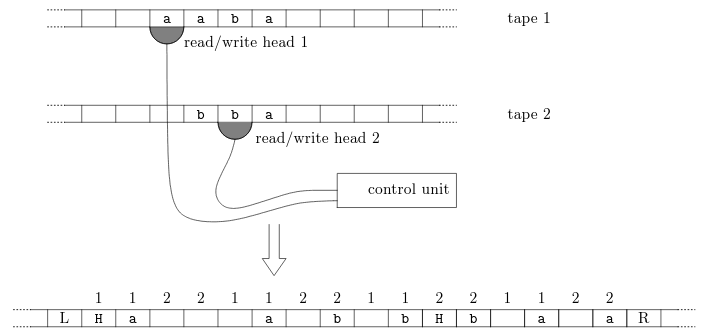
\includegraphics[width=0.9\textwidth]{two_tape_turing_machine}
		\caption{How to simulate a two tape Turing machine on a single tape machine}
		\label{fig:two tape turing machine}
	\end{figure}
	
	\subsubsection{Multidimensional Tapes}
	Now we consider a tape where the Turing machine can move not just left and right, but also up and down for a two dimensional machine. This offers more than a multitape machine as each row can be considered as its own individual tape and the machine now has an unbounded amount of tapes available at its disposal. Once again this does not add any computing power, just convenience to the machine, as we can simulate this using two one-dimensional tapes which we can then simulate on a single tape.
	
	
	\subsubsection{The Universal Turing Machine}
	We can build a Turing machine which takes as input an arbitrary transition table and some data which it can then simulate the behaviour of. Turing realised the practical importance of this idea: instead of building new machines each time a new task is being tackled, we can instead program the universal Turing machine\index{universal turing machine} to do the job at hand. In other words, this embodies the idea of the \textit{stored program}, now associated with von Neumann. 
	
	\subsection{Church's Thesis}
	\begin{theorem} 
		What ever can be done by any computational device can be done by a Turing machine
	\end{theorem}
	
	\par Church's thesis cannot be proven - it's entirely possible for someone to invent a new way of computation which extends the capabilities of programs as we know them. All variations of Turing machines that we have seen have no more computational power than the base Turing machine. On the other hand, nobody has been able to come up with an alternative to Turing machines as of yet and the more time that passes the more plausible Church's thesis becomes.
	
	\section{Complexity and P}
	Until now we have been concerned with figuring out what a computer can and can't do. According to Church's thesis, this distinction of what we can and can't do does not depend at all on the architecture of the machine or the programming language - it's a fundamental divide. We have also seen that there are problems of practical intrest which exceed the capabilities of computers. These problems we can only solve approximately or partially. This section is concerned with classifying problems according to the computational effort they need for their solution. There are many different ways to accomplish this. In the simplest case we will look at decision problems which require a yes/no answer.
	
	\par 
	In computer science we use the term \textbf{complexity}\index{complexity} differently than we do in English where it normally means 'multi-faceted' or 'confusing'. In the study of programs we use the word strictly to refer to the amount of resources needed during computation - primarily \textbf{time} and \textbf{space}. In select other cases we may be interested in other resources such as number of file accesses. We also must make the distinction between the complexity of an algorithm (which we have studied before and refers to the runtime behaviour of a program) and the complexity of a problem which refers to an inherent difficulty in solving a problem. 
	
	\par 
	We study the runtime of Turing machines rather than any real computer. This is for a number of reasons. Firstly, the time and Turing machine takes is unambiguously characterised by the number of transitions it makes allowing us to not have to bring in actual time measurements. Secondly, the space usage of a Turing machine can be defined unambiguously as well. We take this to be the number of cells it ever visits during computation. As tape cells have finite capacity only, this measure is fair and realistic. Thirdly, Turing machines operate uniformly on input of arbitrary size. A Turing machine will behave the same regardless of if a string is two characters long or two billion characters long which is not true of real hardware. Turing machines can scale up in size, real computer programs typically don't.
	
	\par 
	Once we have designed a Turing machine to solve a particular problem, how do we find the time complexity of the program? It is not sufficient to test the program on a few strings and just tabulate the outcomes. We would really like to give the number of steps executed by the machine for all possible inputs it can take - this is the function from the input domain (for example $\Sigma^{*}$, strings over $\Sigma$) to the set of natural numbers. Such a formula is probably very difficult to find for even the most simple Turing machines. It is also not clear whether we can read off a lot from the formula should we find it.
	
	\par If we abstract away from the actual input to the length of the input, the situation becomes much more manageable both in terms of finding the formula and in terms of interpreting the given formula. Mathematically, we will get a function from the natural numbers (the input length) to the natural numbers (number of steps taken). It's important to be precise about how the abstraction is achieved. We may associate the input length $n$ with $n^{2}$ if the Turing machine takes at most $n^{2}$ steps. This is very different to interpretting $n^{2}$ as the number of steps on average. We can distinguish three cases when analysing the runtime complexity of an algorithm:
	\begin{itemize}
		\item \textbf{Best-case runtime} or \textbf{Minimum time}: The time needed when the algorithm is applied to the 'easiest' possible input. An example is applying a sorting algorithm to the already sorted list.
		\item \textbf{Worst-case runetime} or \textbf{Maximum time}: The time needed when the algorithm is applied to the 'worst' possible input. An example is applying a sorting algorithm to a list sorted in reverse order.
		\item \textbf{Average-case runtime} or \textbf{Average time}: The average time needed (where the average is taken over all possible inputs).
	\end{itemize}
	
	\par 
	We known how to determine the time-complexity of algorithms from first-year. We now take one further abstraction and ask whether problems themselves have an inherent complexity? In general the answer to this question is sometimes 'yes', sometimes 'yes but currently unknown' and sometimes 'no'. We are trying to make a statement about all algorithms which would solve the problem by assigning a complexity to a problem. This idea can fail in practice in a number of ways.
	\begin{enumerate}
		\item We can have a situation where we suspect that the problem is solvable but nobody has been able to give an algorithm for it yet.
		\item We may have one or a number of algorithms but we are unable to determine their complexity functions. This was the case for the Simplex Method\index{simplex method}.
		\item We may have a few algorithms and we may know their complexity but we do not know whether there exist better algorithms or not.
		\item We may have the situation that there are probably better and better algorithms for a given problem, we can then never determine the largest lower bound of the complexity.
	\end{enumerate}
	Cases 1 and 2 are rare but have some spectacular examples. Case 4 seems to only occur in problems that have been designed specifically for that purpose. Case 3 is the most common situation. The most common example of case 3 is that we know we can solve the Travelling Salesman problem in exponential time but we don't know if there exists a more efficient algorithm. In general, for every specific algorithm, whose runtime behaviour is known, gives us an \textit{upper bound} for the complexity of a problem (like saying I know I can do this in f(n) many steps, but maybe we can do better). A \textit{lower bound} cannot be established by programming at all, instead you need a clever way of analysing the problem which shows that every algorithm must take atleast so many steps. For many problems, we don't have lower bounds yet and they are very challeging to come across.
	
	\subsection{The complexity class $\mathcal{P}$}
	For the problem of copying a string on a one-tape Turing machine, we can show that every implementation will have a time complexity which is at least quadratic. However, when we change to a two tape scenario we can achieve a much faster implementation which runs in linear time. Because of this, should we religiously stick to one tape machines, or should we be more liberal in our choice of machine? What this example shows us is that we need to say which machine model we are referring to - by convention this is the multitape Turing machine.
	
	\par Are there complexity classes which are independent of the machine model? Absolutely. Problems which have a polynomial complexity on Turing machines (problems whose complexity class is $O(n^{k})$ have polynomial complexity on almost all machine models. A machine model is 'reasonable' only if it defines the same class of polynomial problems as Turing machines. The class of polynomial problems with polynomial implementations is denoted by $\mathcal{P}$ and it is customary to call the problems in $\mathcal{P}$ \textbf{feasible}\index{feasible} and those outside \textbf{infeasible}\index{infeasible} or \textbf{intractable}\index{intractable}.
	
	\section{NP}
	We have introduced the distinction between problems which have a solution which runs in polynomial time and problems for which a solution does not exist. The former problems are \textbf{feasible}\index{feasible} and the latter are \textbf{intractable}\index{intractable}. We use $\mathcal{P}$ to notate all problems which are feasible.
	
	\par 
	The distinction between $\mathcal{P}$ and not-$\mathcal{P}$ is not easy to establish in practice.
	
	\par 
	There is a whole range of very common problems which are not sure if they are feasible or not. These are called \textbf{$\mathcal{NP}$-complete problems}. In a nutshell, for $\mathcal{NP}$-complete problems we do not know whether the problems are really hard, but we have very good grounds to believe it.
	
	\par 
	The easiest way to explain the class $\mathcal{NP}$ is via the distinction between solving a problem and checking a solution. From experience, we know that checking a solution is much easier than solving a problem. $\mathcal{NP}$ consists of all the problems for which there exists a polynomial solution checking algorithm. For example, it is very easy to check that a number is divided by another, no matter how large the numbers are. On the other hand, finding a factor of a given number - even if you know if the number is prime or not - is very hard to do. RSA encryption is built upon this fact, and solving the problem would have profound effects. 
	
	\par 
	The formal definition of what it means to check a solution is a little involved. This is because each instance may require additional data to do the checking efficiently, having the answer alone may not be enough. We will look at decision problems where the answer is either 'yes' or 'no'. Such an answer does not make it any easier to check whether it is correct or not. We need something additional, which we call a \textbf{proof}\index{proof} or a \textbf{witness}\index{witness}. In the division example this would be the factors of the number (which gives us more information that just that the number is composite). The checker can then verify the answer by multiplying the factors together. We formalise this idea of a witness:
	\begin{definition}
		A subset $L$ of $\Sigma^{*}$ belongs to $\mathcal{NP}$ if there exists a determinisitc Turing machine $M$ which takes pairs $(s, w)$ of strings as input and replies 'yes' or 'no' in polynomial time. The replies are to be interpretted as saying 'yes, $w$ proves that $s$ belongs to $L$' or 'no, this $w$ is not a proof for the membership of $s$ in $L$. Furthermore, it must be true that for every $s \in L$ there exists at least one witness $w \in \Sigma^{*}$ such that $M$ will reply 'yes' when presented with $(s, w)$ and for every $s \in L$ no witness exists for which $M$ replies 'yes'.
	\end{definition}
	
	\subsection{Nondeterministic Turing Machines}
	We can define the class $\mathcal{NP}$ is a completely different way using \textbf{nondeterministic Turing machines}. NTMs are defined just like determinisitic Turing machines expect we use a transition \textit{relation} rather than a transition \textit{function}. In essence, we get a transition table where every entry consists of finitely many choices for how the machine may proceed and the machine is allowed to choose freely at every stage one of the transistions from the available collection.
	
	\par 
	We will concentrate our efforts on decision problems once again. When we design an NTM for a decision problem it makes sense to allow for a third possible outcome: 'undecided' or 'can't make a judgement either way'. The machine is \textbf{correct} if it never replies 'yes' when it should have said 'no' and if it never replies 'no' when it should have said 'yes'. In all cases it is allowed to respond with 'undecided'. An NTM is said to \textbf{solve} a decision problem if it is correct and for every positive instance there is at least one computation path along which the machine will reply 'yes'.
	
	\par 
	We can use an NTM to construct a deterministic machine which truly decides the decision problem (although it takes a long time to do so). The determinisitic machine systematically explores all execution paths the nondeterministic machine is capable of. As the NTM is bound to stop after a fixed amount of time, there is only finitely many paths to consider. If one branch ends with 'yes' then the determinisitic machine answers 'yes' as well. If all branches end in 'undecided' or one branch answers 'no', the deterministic machine answers 'no'.
	
	\par 
	The worst case complexity of a NTM is defined almost as in the determinisitic case: we take the maximum run time (or memory usage) on all input of a certain length, and for all possible choices the machine can make. Their runtime is bounded by some polynomial independently of the choices they can make during a computation.
	
	\begin{definition}
		A decision problem belongs to the complexity class $\mathcal{NP}$ if there exists a nondeterminisitic Turing machine running in polynomial time solving the problem.
	\end{definition}
	
	The second definition makes it easier to see that $\mathcal{P}$ is contained in $\mathcal{NP}$ because deterministic Turing machines are also NTMs. The question of whether the two classes are different or not is a famous open question in the theory of computation, commonly referred to as the $\mathcal{P} = \mathcal{NP}$ problem.
	
	\subsection{Complete Problems}
	Some problems in NP have been studied for hundreds of years and yet no efficient solution has been found. This suggests that $\mathcal{NP}$ is a larger class of problems than $\mathcal{P}$. It's reasonable to prove this idea by selecting some hard problem in $\mathcal{NP}$ and showing a lower bound for it which grows faster than any polynomial. To do this, we need an alternative notion of comparing problems in a single complexity class. For $\mathcal{NP}$ this idea of comparisson is given by \textbf{polytime reducability}\index{polytime reducability}. We say a problem $\mathcal{X}$ reduces in polynomial time to a problem $\mathcal{Y}$ if there is an algorithm (determinisitic Turing machine) which translates instances of $\mathcal{X}$ to instances of $\mathcal{Y}$ whose runtime is polynomial bounded. We write $\mathcal{X} \leqp \mathcal{Y}$ for this relationship. If $\mathcal{X}$ and $\mathcal{Y}$ are in $\mathcal{NP}$ and if $\mathcal{X}$ can be reduced to $\mathcal{Y}$ in polynomial time then it is reasonable to say that $\mathcal{X}$ is 'eaiser' than $\mathcal{Y}$ because any polynomial Turing machine solving $\mathcal{Y}$ also gives a solution to $\mathcal{X}$.
	
	\par 
	It is the case that there are some nontrivial reductions between problems within $\mathcal{NP}$ and it could be the case that $\mathcal{NP}$ as a whole consists of infinitely many layers of problems, each more difficult than the one that precedes it. Becuase of this, it is remarkable that $\mathcal{NP}$ contains problems that are maximally difficult, in the sense that every other $\mathcal{NP}$ problem can be reduced to them. These problems are called \textbf{complete for $\mathcal{NP}$ with respect to polytime reductions}, or for short \textbf{$\mathcal{NP}$-complete}\index{NP-complete}.
	
	
	\subsection{Examples of NP-complete problems}
	\subsubsection{SAT}
	The satisifiability of propositional expressions (SAT) is a $\mathcal{NP}$-complete problem. Propositional formulae are generated by the following grammar:
	\begin{align*}
	\phi &::= A \;| \; \bot \;|\; \top \;|\; \phi \wedge \phi \;|\; \phi \vee \phi \;|\; \neg \phi \;|\; \phi \rightarrow \phi \\
	A &::= p \;|\;q \;| \; r ...
	\end{align*}
	
	Here $p, q, r$ are the propositional variables - placeholders for either true or false. The satisfiability problem consists of deciding for a given propositional formula whether there exists an assignment of truth values to atomic formulas such that the given formula becomes true as a whole. $\neg(q \rightarrow p) \wedge $ becomes true when $p$ is false and $q, r$ are true. 
	
	\par 
	We have to say how a Turing machine would deal with propositional formulae. We have an input alphabet $\Sigma = \{p, \top, \bot, \neg, \vee, \wedge, \rightarrow, \leftrightarrow, \left(, \right), 0, 1\}$. We have one letter for propositional variables - we use 0 and 1 to generate infinitely many expressions consisting of $p$ followed by a binary digit. Using this alphabet, we can encode formulae as strings with an unambiguous definition of the length of the formula. SAT certainly belongs in $\mathcal{NP}$ as the NTM will simply guess some assignment of truth values to propositional variables and then evaluate the expression.
	
	\par 
	In 1971, Stephen Cook proved that SAT is an $\mathcal{NP}$-complete problem. To prove this, we have to show an arbitrary problem in $\mathcal{NP}$ can be reduced to a satisfiability problem. The only definite information we have about $\mathcal{NP}$-problems is that they are decided by polynomial time NTMs - the proof relies upon this fact.
	
	\subsubsection{Others}
	In Graph Theory, deciding whether a given graph contains a closed path (a cycle) which visits every node exactly once. This is the \textbf{Hamiltonian Path Problem}\index{hamiltonian path problem}. In discrete optimisation, deciding whether a given graph contains a cycle which visits every node at least once, and along which the weights add up to less than a given constant $K$ (otherwise known as the \textbf{Travelling Salesman Problem}\index{travelling salesman problem}). Deciding whether a set of tasks can be scheduled on two processors in such a way that all tasks are completed by a given deadline is also an $\mathcal{NP}$-complete problem. 
	\par 
	Interestingly, finding the factors of a natural number, while clearly in $\mathcal{NP}$ does not appear to be an $\mathcal{NP}$-complete problem. Currently there is no proof for this.
	
	\section{Lambda-calculus}
	Alonzo Church developed a notation for arbitrary \textbf{functions} called $\lambda$-calculus. It is an extremely economical notation but at first sight somewhat cryptic, which stems from its origins in mathematical logic. Expressions in $\lambda$-calculus are written in strict prefix form. Further, function and argument are simply written next to each other without brackets around the argument.
	
	\subsection{$\delta$-reduction}
	$\delta$-reductions are equivalent to ordinary arithmetic expressions. 
	\[ \underline{m} + \underline{n} \leadsto_{\delta} \underline{m + n}\]
	
	For example:
	\[ \underline{5} + \underline{7} \leadsto_{\delta} \underline{12} \]
	\subsection{$\beta$-reduction}
	$\beta$-reductions can be thought of substituting arguments into a function.
	
	\[(\lambda x . \; M) \; N \leadsto_{\beta} M[N/x] \]
	
	Here, $M$ is the body of the $\lambda$-abstraction, $N$ is the argument and $M[N/x]$ means $M$ where we have replaced $x$ by $N$.
	
	\[(\lambda x . \; x + \underline{3}) \; \underline{7} \leadsto_{\beta} \underline{7} + \underline{3} \leadsto_{\delta} \underline{10} \]
	\subsection{$\alpha$-reduction}	
	$\alpha$-reduction allows bound variable names to be changed. Example:
	\begin{align*}
	\lambda x . \; (\lambda x . \; x) &\leadsto_{\alpha} \lambda y . \; (\lambda x . \; x) \\
	 &\leadsto_{\alpha} \lambda y . \; (\lambda x . \; y) \qquad \text{WRONG}
	\end{align*}
	
	When substituting values, we need to be careful. 
	\begin{align*}
	(\lambda x . \; ((\lambda x . \; x) \; \underline{17}) \; + x) \; &\underline{8} \\
	\leadsto \; ((\lambda x . \; \underline{8}) \; \underline{17}) \; + &\underline{8} \qquad \text{WRONG} \\
	\leadsto \; ((\lambda \underline{8} . \; \underline{8}) \; \underline{17} ) \; + &\underline{8} \qquad \text{WRONG}
	\end{align*}
	
	When we form $M[N/x]$, we replace only the free occurances of $x$ by $N$.
	
	Take the following terms:
	\begin{align*}
		\lambda x .\quad \lambda x.\quad \lambda y .\quad &x + \underline{3} \\
		\lambda u . \quad \lambda v. \quad \lambda u . \quad &v + \underline{3}
	\end{align*}

	These two terms are $\alpha$-equivalent\index{alpha equivalent}. We say two terms are $\alpha$-equivalent when they are the same except for the binders and the bound occurances of variables, and the variables are bound to the same place. $\alpha$-equivalent terms are regarded as exactly the same.
	
	\subsection{Church-Rosser Theorem}
	\begin{theorem}[Church-Rosser Theorem]
	If a term M can be reduced (in several steps) to terms N and P, there there exists a term Q to which both N and P can be reduced (in several steps)
	\end{theorem}

	\par This is sometimes known as confluence. Regardless of the order in which we decide to reduce our lambda calculus expression, we will always be able to arrive at the same term. This makes perfect sense - when evaluating an expression with arithmetic terms, we cannot get two different answers dependent on the order of evaluation. It follows that we get this corollary:	
	
	\begin{corollary}
	Every $\lambda$-term has at most one normal form.
	\end{corollary}
	
	\par
	We can prove this. Assume there are two normal forms (for the case of contradiction) N and P to which are certain term M reduces. By the theorem of Church and Rosser there is a term Q to which both N and P can be reduced to. However, as we have assumed N and P are in their normal forms they don't allow any further reductions. The only possible interpretation for this is that N = P = Q.
	
	\subsection{Typed Lambda-calculus}
	Currently there is nothing in the grammar of lambda calculus that restricts us from forming awful terms. It would be completely possible to form $\sin \log$ at the moment - the sine function applied to the logarithm function. This is obviously impossible and any programming language would reject this as incorrectly formed. We are currently missing the notion of types, which represent what kind of arguements the function will accept and what it expects to return.
	
	\par 
	We can form the language for expressing these types very easily. We begin with base types such as \texttt{int} and \texttt{real}. On top of this we then form function types. This gives us the following grammar which is called the \textbf{system of simple types}\index{system of simple types}:
	
	\[ \tau ::= c \; | \; \tau \rightarrow \tau \]
	
	\par In this grammar, the value c is used as a placeholder for all of our base types we wish to include. Now we can form function types, we would give the type of the sine function as $\texttt{real} \rightarrow \texttt{real}$, which makes it obvious that it cannot accept the logarithm function as an argument. Using the type system that we have defined, we can create restrictions on what kind of terms are valid (or \textbf{well-typed}). We do this by an inductive definition:
	\begin{itemize}
		\item \textbf{Base Case}: For every type $\sigma$ and every variable $x$, the term $x:\sigma$ is well typed and has type $\sigma$.
		\item \textbf{Function formation}: For every term $M$ of type $\tau$, every variable $x$, and every type $\sigma$, the term $\lambda x:\sigma .M$ is well-typed and has type $\sigma \rightarrow \tau$
		\item \textbf{Application}: If $M$ is well-typed of type $\sigma \rightarrow \tau$ and $N$ is well-typed of type $\sigma$ then $M N$ is well-typed and has type $\tau$
	\end{itemize}	
	
	
	\newpage
	\printindex
\end{document}
